\documentclass[a4,11pt,epsf, amssymb]{article}
\usepackage{color}
\usepackage{graphicx}
\usepackage{rotating}
%\input{../../Yuan/psfig.sty}
\usepackage{amsmath,amsfonts,latexsym,amssymb}
\usepackage{mathrsfs}
    \setlength{\textwidth}{6in}
    \setlength{\textheight}{8in}
    \setlength{\oddsidemargin}{0in}
    \setlength{\topmargin}{0in}
\def\ditem{\vspace{-0.1cm} \item}
%\setcounter{page}{2458}

\usepackage{multirow}
\usepackage{rotating}
\usepackage{caption}
\usepackage{graphicx}
\usepackage{indentfirst}
\usepackage{CJK}

\renewcommand{\baselinestretch}{1.2}


\begin{document}
\begin{CJK}{GBK}{song}
\begin{center}
{\bf\huge Testing the Association between Two Ordinal Variables with Adjusting for Covariates}
\end{center}

\section{Introduction}
Ordinal variable has always gotten great attention in biomedical research. Among all the issues about ordinal variable, testing the association between two ordinal variables with adjusting for covariates is an important one. Testing whether two ordinal variables are related is an common issue and there have been many test statistics measuring the association between two ordinal variables, such as Kruskal`s gamma statistic, the Wilcoxon statistic, the Kruskal-Wallis statistic and the Jonckheere-Terpstra statistic. All these statistics only measuring the association between the two ordinal variables we are interested in regardless of the effect of other covariates. However, sometimes we need to test this kind of association with adjusting for other covariates. On the one hand, there are many practical problems of this type. For example, if we want to test whether smoking and lung cancer are related when other covariates, such as sex and age, have been adjusted, we need to solve this issue. On the other hand, adjusting for other covariates can be more powerful in testing the null hypothesis of no association between the two ordinal variables, especially when other covariates are related with at least one of the two ordinal variables. For example, if we want to test whether smoking and lung cancer are related, the test statistic coming from the logistic regression model is more powerful when we adjust for the covariate such as age, since age can affect the probability of getting cancer. So special attention should be paid to the issue of testing assocaition between two ordinal variabled with adjusing for covariates.

There have been many papers focusing on this issue. Using the proportional odds model is a widely acknowledged method, but it has its own defects. Proportional odds model treat the value of ordinal variables as numeric value. That is, in ordinal variables, this model sets the distance of 1 and 2 the same as that of 2 and 3, which is obvious unfounded in real situation. To solve this problem, we propose a new method for this issue. In our method, we do not use the value of the ordinal variables. Instead, we bring in a latent variable which follows multivariate normal distribution to picture the relationship between all the variables, including the two ordinal variables and other covariates. The normality assumption is reasonable since it is the most common one in real life. We made simulations to compare the proportional odds model method and the new method. It is shown that our new method have less type I error and greater power.

\section{Method}

\subsection{Notations}
Suppose that $X$ and $Y$ are two ordinal variables with $k$ and $m$ categories, respectively. Denote the categories of $X$ and $Y$ by $a_1,a_2,\cdots,a_k$ with $a_1<a_2<\cdots<a_k$
and $b_1,b_2,\cdots,b_m$ with $b_1<b_2<\cdots<b_m$, respectively. Let ${\bf Z}=(Z_1,Z_2,\cdots,Z_L)^\tau$ be a $L$-dimensional continuous covariate. We want to detect the association between $X$ and $Y$ after adjucting for ${\bf Z}$.
The null hypothesis is
$$H_{01}:\hbox{Pr}(X,Y|{\bf Z})=\hbox{Pr}(X|{\bf Z})\hbox{Pr}(Y|{\bf Z}).$$
Let $\{x_1,x_2,\cdots,x_n\}$, $\{y_1,y_2,\cdots,y_n\}$ and $\{{\bf z}_1,{\bf z}_2,\cdots,{\bf z}_n\}$ be the $n$ observations of $X$, $Y$ and ${\bf Z}$, respectively.

\subsection{Models}
Suppose that $X$, $Y$ and ${\bf Z}$ come from a $L+2$-dimensional multi-normal variable ${\bf U}=(U_1,U_2,\cdots,U_{L+2})^\tau$ with zero-vector mean and the variance and covariance matrix $\Delta$, where
$\Delta=(\delta_{l_1l_2})_{(L+2)\times(L+2)}$ and $\delta_{ll}=1$ for $l=1,2,\cdots,L+2$. The covaraites ${\bf Z}=(U_3,U_4,\cdots,U_{L+2})^\tau$, and $X$ and $Y$ are obtained based on the following strategies
$$
X=\left\{\begin{array}{ll}
a_1 & -\infty < U_1 \leq \xi_1\\
a_2 & \xi_1 < U_1 \leq \xi_2\\
\ldots & \ldots\\
a_k & \xi_{k-1} < U_1<\infty;
\end{array}\right.
$$
and
$$
Y=\left\{\begin{array}{ll}
b_1 & -\infty < U_2 \leq \eta_1\\
b_2 & \eta_1 < U_2 \leq \eta_2\\
\ldots & \ldots\\
b_m & \eta_{m-1} < U_2< \infty.
\end{array}\right.
$$
where $-\infty<\xi_1<\xi_2<\cdots<\xi_{k-1}<\infty$ and $-\infty<\eta_1<\eta_2<\cdots<\eta_{m-1}<\infty$.


Denote
$$\Delta=\left(\begin{array}{cc}\Delta_{11}&\Delta_{12}\\ \Delta_{21}&\Delta_{22}\end{array}\right),$$
where $\Delta_{11}$ is a 2 by 2 matrix. Then
$$(U_1,U_2|{\bf Z})^\tau \sim N \left(\Delta_{12}\Delta_{22}^{-1}{\bf Z}, \Delta_{11}-\Delta_{12}\Delta_{22}^{-1}\Delta_{21}\right).$$
Denote $\delta=(\delta_{12},\delta_{13},\cdots,\delta_{1(L+2)},\delta_{23},\delta_{24},\cdots,\delta_{2(L+2)},\cdots,\delta_{(L+1)(L+2)})^\tau,
\zeta_1 = (\delta_{13}, \delta_{14},\cdots, \delta_{1(L+2)})^{\tau}, \zeta_2 = (\delta_{23}, \delta_{24}\cdots, \delta_{2(L+2)})^{\tau},$ then
\begin{align*}
\Delta_{11}-\Delta_{12}\Delta_{22}^{-1}\Delta_{21} & = \left(\begin{array}{cc} 1 &\delta_{12}\\ \delta_{12}& 1\end{array}\right) - \left(\begin{array}{c} \zeta_1^\tau \\ \zeta_2^\tau \end{array} \right) \Delta_{22}^{-1} (\zeta_1,\zeta_2)\\
& = \left(\begin{array}{cc} 1 - \zeta_1^\tau \Delta_{22}^{-1} \zeta_1 & \delta_{12} - \zeta_1^\tau \Delta_{22}^{-1} \zeta_2 \\
\delta_{12} - \zeta_2^\tau \Delta_{22}^{-1} \zeta_1 & 1 - \zeta_2^\tau \Delta_{22}^{-1} \zeta_2 \end{array} \right)
\end{align*}
Denote $\varrho(\delta) = \delta_{12} - \zeta_1^\tau \Delta_{22}^{-1} \zeta_2$. Then testing $H_{01}$ is equvalent to test
$$H_{02}:\varrho(\delta) = 0.$$
Now we need to estimate the value of $\delta_{12},\zeta_1,\zeta_2,\Delta_{22}.$\\

From
$$(U_1,{\bf Z}^\tau)^\tau \sim N \left(\left(\begin{array}{c} 0 \\ 0_{L\times1}\end{array}\right),\left(\begin{array}{cc}1 & \zeta_1^\tau \\ \zeta_1 & \Delta_{22} \end{array}\right)\right)$$
we get the conditional distribution of $U_1$ when $\bf Z$ is given,
$$(U_1|{\bf Z}) \sim N(\zeta_1^\tau\Delta_{22}^{-1}{\bf Z}, 1-\zeta_1^\tau\Delta_{22}^{-1}\zeta_1)$$
Similarly, from
$$(U_2,{\bf Z}^\tau)^\tau \sim N \left(\left(\begin{array}{c} 0 \\ 0_{L\times1}\end{array}\right),\left(\begin{array}{cc}1 & \zeta_2^\tau \\ \zeta_2 & \Delta_{22} \end{array}\right)\right)$$
we get the conditional distribution of $U_2$ when $\bf Z$ is given,
$$(U_2|{\bf Z}) \sim N(\zeta_2^\tau\Delta_{22}^{-1}{\bf Z}, 1-\zeta_2^\tau\Delta_{22}^{-1}\zeta_2)$$
Denote $\xi_0=-\infty, \xi_k=\infty,\eta_0=-\infty, \eta_m=\infty$. Then the marginal density functions have the following form
%\begin{equation}
\begin{align*}
f_1(X,Y,\delta_{12},u_i) & = \prod_{1\leq i \leq k \atop 1\leq j \leq m}\left[\int_{\eta_{j-1}}^{\eta_j} \int_{\xi_{i-1}}^{\xi_i}\frac 1{2\pi \sqrt{1-\delta_{12}^2}}\rm e^{-\frac {u_1^2 - 2\delta_{12}u_1u_2 + u_2^2}{2(1-\delta_{12}^2)}}\rm du_1 \rm du_2 \right]^{\rm I(X = a_i, Y=b_j)}  \tag{$1$} \\
f({\bf Z},\Delta_{22}) & = \frac 1{(2\pi)^{\frac L2}|\Delta_{22}|}\rm exp{(-\frac {{\bf Z}^\tau \Delta_{22}^{-1}{\bf Z}}{2})}  \tag{$2$}\\
f_2(X,{\bf Z}, \zeta_1) & = f({\bf Z})f(X|{\bf Z}) \\
 & = \frac 1{(2\pi)^{\frac L2}|\Delta_{22}|}\rm exp{(-\frac {{\bf Z}^\tau \Delta_{22}^{-1}{\bf Z}}{2})}\prod_{j = 1}^k\left[\int_{\xi_{j-1}}^{\xi_j}\frac 1{\sqrt{2\pi(1-\zeta_1^\tau\Delta_{22}^{-1}\zeta_1)}}\rm exp{(-\frac {(u_1 - \zeta_1^\tau\Delta_{22}{\bf Z})^2}{2(1-\zeta_1\Delta_{22}^{-1}\zeta_1)})}\rm du_1\right]^{\rm I(X=a_j)}  \tag{$3$}\\
f_3(Y,{\bf Z}, \zeta_2) & = f({\bf Z})f(Y|{\bf Z}) \\
 & = \frac 1{(2\pi)^{\frac L2}|\Delta_{22}|}\rm exp{(-\frac {{\bf Z}^\tau \Delta_{22}^{-1}{\bf Z}}{2})}\prod_{l = 1}^m\left[\int_{\eta_{l-1}}^{\eta_l}\frac 1{\sqrt{2\pi(1-\zeta_2^\tau\Delta_{22}^{-1}\zeta_2)}}\rm exp{(-\frac {(u_2 - \zeta_2^\tau\Delta_{22}{\bf Z})^2}{2(1-\zeta_2\Delta_{22}^{-1}\zeta_2)})}\rm du_2\right]^{{\rm I}(Y=b_l)}  \tag{$4$}
\end{align*}
%\end{equation}
And the joint distribution of $X,Y,\bf {Z}$ can be approximated by
\begin{equation*}
f(X,Y,{\bf Z}, \delta_{12},\zeta_1,\zeta_2) = f_1(X,Y,\delta_{12})f_2(X,{\bf Z}, \zeta_1)f_3(Y,{\bf Z}, \zeta_2) \tag{$5$}
\end{equation*}

\subsection{Method}
Suppose there are $n$ observations denoted as $\{(x_i,y_i,{\bf z}_i),i=1,\cdots,n\}$ in the sample. The process of estimating $\delta_{12} - \zeta_1^\tau \Delta_{22}^{-1} \zeta_2 $ is as follows:
\begin{enumerate}
    \item In our model, $X$ and $Y$ are ordinal variables that both come from standard normal distribution. So we can use the distribution of $X$ and $Y$ to estimate $\{\xi_j,j=1,\cdots,k-1\}$ and$\{\eta_l,l=1,\cdots,m-1\}$, respectively. That is, denote the numbers of $a_j$ as $u_j$ and that of $b_l$ as $v_l$, $j = 1,\cdots,k,l=1,\cdots,m$. Then the estimators of $\{\xi_j,j=1,\cdots,k-1\}$ and$\{\eta_l,l=1,\cdots,m-1\}$ are the roots of the following equations, which are denoted as $\{\hat{\xi}_j,j=1,\cdots,k-1\}$ and$\{\hat{\eta}_l,l=1,\cdots,m-1\}$
        \begin{align*}
        u_j & = \Phi(\hat{\xi}_j) - \Phi(\hat{\xi}_{j-1}),j = 1,\cdots,k-1 \\
        v_l & = \Phi(\hat{\eta}_l) - \Phi(\hat{\eta}_{l-1}), l= 1, \cdots, m-1
        \end{align*}
        Denote $P_{jl} = P(X=a_j,Y=b_l) = \int_{\hat{\eta}_{l-1}}^{\hat{\eta}_l} \int_{\hat{\xi}_{j-1}}^{\hat{\xi}_j}g(u_1,u_2) \hbox{d}u_1 \hbox{d}u_2$, where
        $$g(u_1,u_2)=\frac 1{2\pi \sqrt{1-\delta_{12}^2}}\rm exp{(-\frac {u_1^2 - 2\delta_{12}u_1u_2 + u_2^2}{2(1-\delta_{12}^2)})}.$$
        So the likelihood function of $\{(x_i,y_i),i = 1,\cdots,n\}$ is
        $$L_1(\delta_{12}) = \prod_{i=1}^n \prod_{j=1,\cdots,k \atop l= 1,\cdots,m}P_{jl}^{\hbox {I}\{x_i = a_j, y_i = b_l\}}.$$
        Maximize $L_1$, we get the maximum likelihood estimator(MLE) of $\delta_{12}$, denoted as $\hat{\delta}_{12}.$
    \item Using the marginal density function (2) for ${\bf Z}$, we have the likelihood function
        $$L_2(\Delta_{22}) = \prod_{i=1}^n f({\bf z}_i,\Delta_{22}) = \frac 1{(2\pi)^{\frac L2}|\Delta_{22}|}\rm exp{(-\frac {{\bf z}_i^\tau \Delta_{22}^{-1}{\bf z}_i}{2})}.$$
        Maximize $L_2$, we get the MLE of $\Delta_{22}$, denoted as $\hat{\Delta}_{22}.$
    \item Plug the estimators $\hat{\xi}_j,j=1,\cdots,k$ and $\hat{\Delta}_{22}$ in the marginal density function (3), we obtain the likelihood function
        $$L_3(\zeta_1)=\prod_{i=1}^n f_2(x_i,{\bf z}_i,\zeta_1).$$
        Maximizing $L_3$ results in the estimator of $\zeta_1$, denoted as $\hat{\zeta}_1.$
    \item Plug the estimators $\hat{\eta}_l,l=1,\cdots,m$ and $\hat{\Delta}_{22}$ in the marginal density function (4), we obtain the likelihood function
        $$L_4(\zeta_2)=\prod_{i=1}^n f_2(x_i,{\bf z}_i,\zeta_2).$$
        Maximizing $L_4$ results in the estimator of $\zeta_2$, denoted as $\hat{\zeta}_2.$
    \item The estimator of $\varrho(\delta)$ is $\hat{\varrho}(\delta) = \hat{\delta}_{12} - \hat{\zeta}_1^\tau \hat{\Delta}_{22}^{-1} \hat{\zeta}_2$
\end{enumerate}

Having estimated $\varrho(\delta)$, we want to obtain the approximate distribution of $\hat{\varrho}(\delta)$ and the Type I error and power of our method. The procedure is as follows:
\begin{enumerate}
    \item Denote $\delta_0 = (\delta_{12},\zeta_1,\zeta_2)$. Using (5), the likelihood function of $\{(x_i,y_i,{\bf z}_i),i=1,\cdots,n\}$ is
    $$L(\delta_0) = \prod_{i=1}^n f(x_i,y_i,{\bf z}_i,\delta_{12},\zeta_1,\zeta_2) = \prod_{i=1}^n \left(f_1(x_i,y_i,\delta_{12})f_2(x_i,{\bf z}_i, \zeta_1)f_3(y_i,{\bf z}_i, \zeta_2)\right).$$
    And the log-likelihood function is
    \begin{align*}
    l(\delta_0) & = \sum_{i=1}^n \log(f(x_i,y_i,{\bf z}_i,\delta_{12},\zeta_1,\zeta_2)) \\
    & = \sum_{i=1}^n (\log(f_1(x_i,y_i,\delta_{12}))+\log(f_2(x_i,{\bf z}_i, \zeta_1))+\log(f_3(y_i,{\bf z}_i, \zeta_2)))
    \end{align*}
    So the $\hat{\delta}_{12},\hat{\zeta}_1,\hat{\zeta}_2$ that we obtained before are also the MLE of the joint distribution of $(X,Y,{\bf Z})$. That is, they are the roots of
    $$\frac{\partial l(\delta_0)}{\partial \delta_0} = 0.$$
    \item Define
        \begin{align*}
        \varphi(X,Y,{\bf Z},\delta_0) & = \frac{\partial \log f(X,Y,{\bf Z},\delta_0)}{\partial \delta_0} \\
        & = \frac{\partial (\log f_1(X,Y,\delta_{12}) + \log f_2(X,{\bf Z},\zeta_1) + \log f_3(Y,{\bf Z},\zeta_2))}{\partial \delta_0} \\
        & = (\frac {\partial \log f_1}{\partial \delta_{12}}, (\frac {\partial \log f_2}{\partial \zeta_1})^\tau, (\frac {\partial \log f_3}{\partial \zeta_2})^\tau )^\tau.
        \end{align*}
        Then
        $$\frac{\partial \varphi(X,Y,{\bf Z}, \delta_0)}{\partial \delta_0^\tau} = \left(\begin{array}{ccc}
        \frac{\partial^2\log f_1}{\partial \delta_{12} \partial \delta_{12}} & \frac{\partial^2\log f_1}{\partial \delta_{12}\partial \zeta_1^\tau} & \frac{\partial^2 \log f_1}{\partial \delta_{12}\partial \zeta_2^\tau} \\
        \frac{\partial^2\log f_2}{\partial \zeta_1 \partial \delta_{12}} & \frac{\partial^2\log f_2}{\partial \zeta_1 \partial \zeta_1^\tau} & \frac{\partial^2\log f_2}{\partial \zeta_1 \partial \zeta_2^\tau}\\
        \frac{\partial^2\log f_3}{\partial \zeta_2 \partial \delta_{12}} & \frac{\partial^2\log f_3}{\partial \zeta_1 \partial \zeta_2^\tau} & \frac{\partial^2\log f_3}{\partial \zeta_2 \partial \zeta_2^\tau} \end{array}\right)\\
        = \left(\begin{array}{ccc}
        \frac{\partial^2\log f_1}{\partial \delta_{12} \partial \delta_{12}} & & \\
        & \frac{\partial^2\log f_2}{\partial \zeta_1 \partial \zeta_1^\tau} & \\
        & & \frac{\partial^2\log f_3}{\partial \zeta_2 \partial \zeta_2^\tau} \end{array}\right),$$
        $$\varphi(X,Y,{\bf Z}, \delta_0)\varphi^\tau(X,Y,{\bf Z}, \delta_0) = \left(\begin{array}{ccc}
        \left(\frac{\partial \log f_1}{\partial \delta_{12}}\right)^2 & \frac{\partial \log f_1}{\partial \delta_{12}}\cdot\frac{\partial \log f_2}{\partial \zeta_1} & \frac{\partial \log f_1}{\partial \delta_{12}}\cdot\frac{\partial \log f_3}{\partial \zeta_3} \\
        \frac{\partial \log f_2}{\partial \zeta_1}\cdot\frac{\partial \log f_1}{\partial \delta_{12}} &
        \left(\frac{\partial \log f_2}{\partial \zeta_1}\right)^2 &
        \frac{\partial \log f_2}{\partial \zeta_1}\cdot\frac{\partial \log f_3}{\partial \zeta_2} \\
        \frac{\partial \log f_3}{\partial \zeta_2}\cdot\frac{\partial \log f_1}{\partial \delta_{12}} &
        \frac{\partial \log f_3}{\partial \zeta_2}\cdot\frac{\partial \log f_2}{\partial \zeta_1} &
        \left(\frac{\partial \log f_3}{\partial \zeta_2}\right)^2 \end{array} \right),$$
        Denote
        \begin{align*}
        I(\delta_0) & = \frac 1n\sum_{i=1}^n \varphi(x_i,y_i,{\bf z}_i, \delta_0)\varphi^\tau(x_i,y_i,{\bf x}_i, \delta_0)\\
        J(\delta_0) & = -\frac 1n\sum_{i=1}^n \frac{\partial \varphi(x_i,y_i,{\bf z}_i, \delta_0)}{\partial \delta_0^\tau}\\
        V(\delta_0) & = J(\delta_0)^{-1}I(\delta_0)J(\delta_0)^{-1}
        \end{align*}
        where $J(\delta_0)^{-1}$ is the reverse matrix of $J(\delta_0).$
        Then using the M-Esitimation method, we know that $\hat{\varrho}(\delta)$ is asymptotically multivariate normal(AMN), that is
        $$\hat{\varrho}(\delta) \quad \hbox {is AMN} \quad \left(\varrho(\delta),\frac{V(\delta_0)}{n} \right) \quad \hbox {as} \quad  n \rightarrow \infty.$$
        Plug in the estimator of $\delta_0$, we have the estimated variance for $\varrho(\delta)$,that is $\frac{V(\hat{\delta}_0)}{n}$. Now we can calculate the p-value of $\varrho(\hat{\delta}).$
\end{enumerate}

\section{Simulation Studies}

In this section, we carried out simulation studies to investigate the performance of our method and to compare it with the approach using the proportional odds model. The first subsection is the simulation for two ordinary ordinal variables. The second subsection is the simulation for two ordinal variables and one of these two variables follows the genetype distribution.
\subsection{Simulation for two ordinal variables}

In this subsection, $X$ and $Y$ are ordinal variables whose values are both in $\{0,1,2,3,4\}$ but follow different distributions, with the former being $\{0.7,0.1,0.08,0.07,0.05\}$ and the latter being $\{0.8,0.08,0.05,0.04,0.03\}$, respectively. $Z$ is a one dimension vector.
The specifics of our data generating scenarios are as follows. We first generated a three dimension vector ${\bf U}$ using the three dimension normal distributions, with mean vector being \{0,0,0\} and variance-covariance matrix being $\Sigma$. $\Sigma$ has the form as
$$\Sigma = \left( \begin{array}{ccc} 1 & r & 0.1 \\ r & 1 & 0.1 \\ 0.1 & 0.1 & 1 \end{array} \right)$$
We change the value of $r$ to change the conditional correlation between $U_1$ and $U_2$. Then we recoded the $U_1$ and $U_2$ as $X$ and $Y$ according to their values.
We set $r$ to be $-0.3, -0.2, -0.1, \\ 0.1, 0.2, 0.3$ to compare the two methods. Besides, we set $\Sigma$ to be
$$\Sigma = \left( \begin{array}{ccc} 1 & 0.4 & 0.5 \\ 0.4 & 1 & 0.8 \\ 0.5 & 0.8 & 1 \end{array} \right)$$
to compare under the null hypothesis.

For each specific conditional correlation coefficient, we generate 1000 datasets, each consisting of $n$ subjects, to obtain the power and type I error of these two methods. The simulation results are summarized in Table 1.\\
\begin{sidewaystable}[!hbp]
\caption{Table 1 power and type I error}
\begin{tabular}{|c|c|c|c|c|c|c|c|c|c|c|c|c|c|c|}

\hline
& \multicolumn{2}{|c|}{$r = -0.3$} & \multicolumn{2}{|c|}{$r = -0.2$} & \multicolumn{2}{|c|}{$r = -0.1$} &
 \multicolumn{2}{|c|}{null hypothesis} & \multicolumn{2}{|c|}{$r = 0.1$} & \multicolumn{2}{|c|}{$r = 0.2$} &
  \multicolumn{2}{|c|}{$r = 0.3$}\\
\hline
n & new & prop & new & prop & new & prop & new & prop &
 new & prop & new & prop & new & prop \\

\hline
250 & 0.854 & 0.747 & 0.534 & 0.382 & 0.209 & 0.135 & 0.061 & 0.06 & 0.144 & 0.146 & 0.484 & 0.462 & 0.809 & 0.804 \\
300 & 0.879 & 0.781 & 0.579 & 0.463 & 0.24 & 0.17 &
0.049 & 0.057 & 0.156 & 0.146 & 0.525 & 0.508 & 0.866 & 0.854\\
350 & 0.939 & 0.889 & 0.639 & 0.518 & 0.24 & 0.167 &
0.063 & 0.059 & 0.159 & 0.162 & 0.565 & 0.547 & 0.911 &  0.908 \\
400 & 0.957 & 0.905 & 0.717 & 0.612 & 0.261 & 0.202 &
0.053 & 0.064 & 0.176 & 0.167 & 0.654 & 0.644 & 0.954 &  0.941 \\
450 & 0.977 & 0.94 & 0.754 & 0.657 & 0.278 & 0.209 &
0.048 & 0.06 & 0.202 & 0.212 & 0.677 & 0.665 & 0.965 &
0.961 \\
500 & 0.988 & 0.97 & 0.784 & 0.71 & 0.331 & 0.253 &
0.042 & 0.059 & 0.225 & 0.216 & 0.743 & 0.721 & 0.988&
0.975 \\
\hline

\end{tabular}
\end{sidewaystable}


From the Table 1, we can see that compared with the method using proportional odds model, our new method has bigger power and smaller type I error in almost all settings.


\subsection{Simulation for genetype variables}

In this subsection, one of the two ordinal variables is genetype variable. A genetype variable is a varible which has three levels with the distribution being $\{(1-p)^2, 2p(1-p), p^2\}$. $p$ is a number betweem 0 and 1, representing the proportion of a gene. In our simulation, $X$ is still a general ordinal varible with five levels, while $Y$ is a genetype varibles, with $p$ changing among $\{0.1, 0.2, 0.3, 0.4, 0.5\}$. With every specific $p$ value, we generate 1000 datasets, each consisting of 1000 subjects to estimate the power and type I error.
The results are summarized in table 2 and the folling Figure1-5.From the table and figures we can see that, when the two ordinal variables are conditional related, our proposed method has bigger power. And at the same time, the new method can control the type I error rate.\\

\begin{table}[!hbp]
\centering
\caption{Table 1 power and type I error}
\begin{tabular}{|c|c|c|c|c|c|c|c|c|c|c|}
\hline
& \multicolumn{2}{|c|}{$r = -0.2$} & \multicolumn{2}{|c|}{$r = -0.1$} & \multicolumn{2}{|c|}{null hypothesis} &
 \multicolumn{2}{|c|}{$r = 0.1$} & \multicolumn{2}{|c|}{$r = 0.2$} \\
\hline
p & new & prop & new & prop & new & prop & new & prop &
 new & prop \\
\hline
0.1 & 0.962 & 0.935 & 0.489 & 0.425 & 0.045 &
0.055 & 0.378 & 0.371 & 0.942 & 0.94   \\
0.2 & 0.995 & 0.992 & 0.639 & 0.584 & 0.039 &
0.037 & 0.471 & 0.458 & 0.975 & 0.968   \\
0.3 & 0.997 & 0.995 & 0.687 & 0.65 & 0.037 &
0.047 & 0.538 & 0.517 & 0.994 & 0.993   \\
0.4 & 0.999 & 0.998 & 0.731 & 0.694 & 0.034 &
0.049 & 0.536 & 0.509 & 0.991 & 0.988   \\
0.5 & 0.998 & 0.998 & 0.741 & 0.714 & 0.033 &
0.036 & 0.582 & 0.559 & 0.991 & 0.992   \\
\hline
\end{tabular}
\end{table}

\begin{figure}
\centering
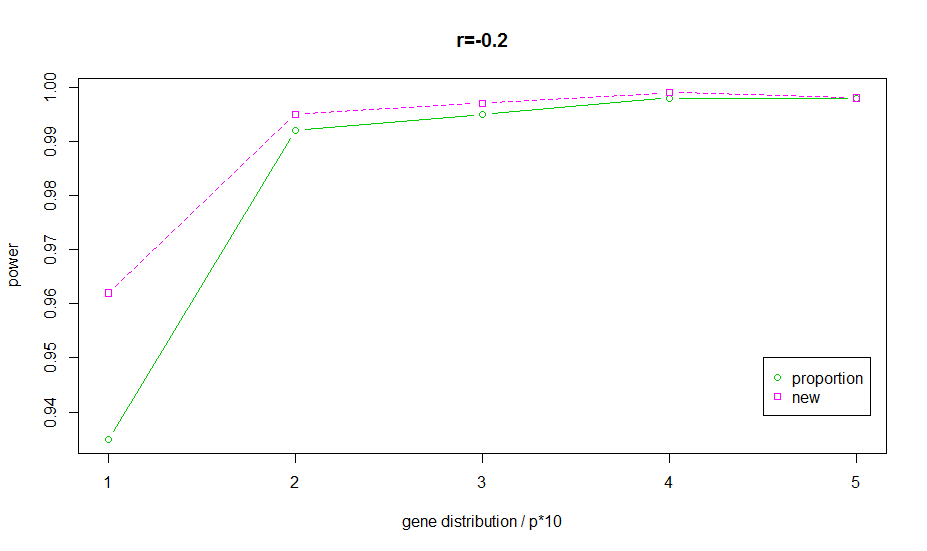
\includegraphics[height = 8cm]{r-2.png}
\caption{$r = -0.2$}
\end{figure}

\begin{figure}
\centering
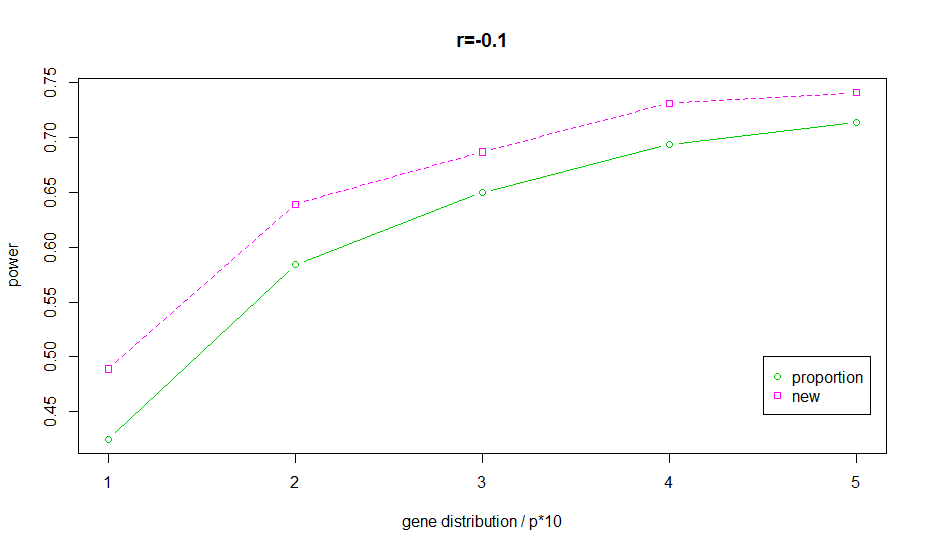
\includegraphics[height = 8cm]{r-1.png}
\caption{$r = -0.1$}
\end{figure}

\begin{figure}
\centering
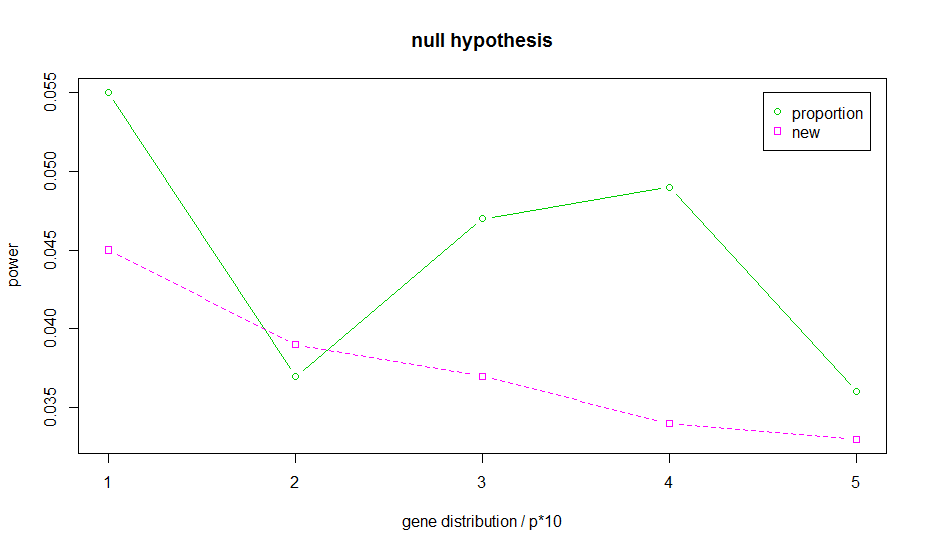
\includegraphics[height = 8cm]{r0.png}
\caption{null hypothesis}
\end{figure}

\begin{figure}
\centering
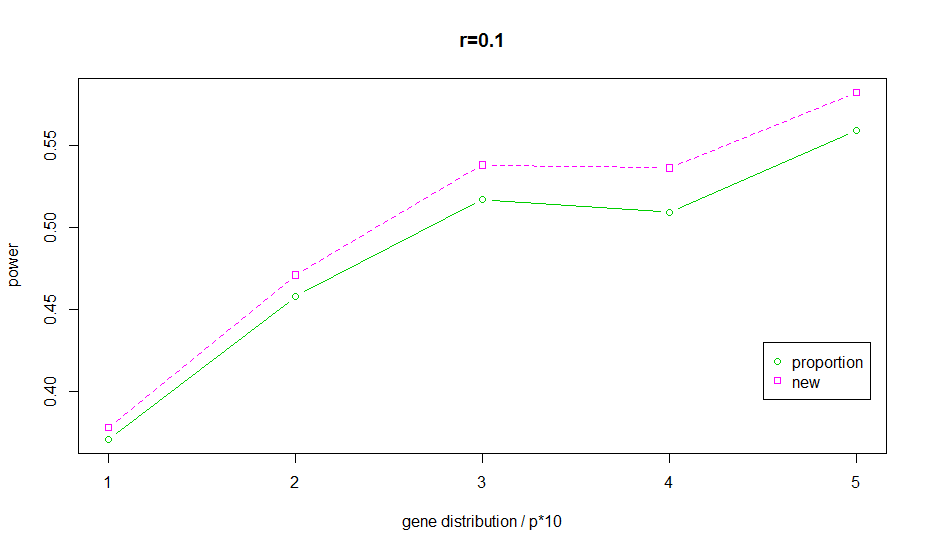
\includegraphics[height = 8cm]{r1.png}
\caption{$r = 0.1$}
\end{figure}

\begin{figure}
\centering
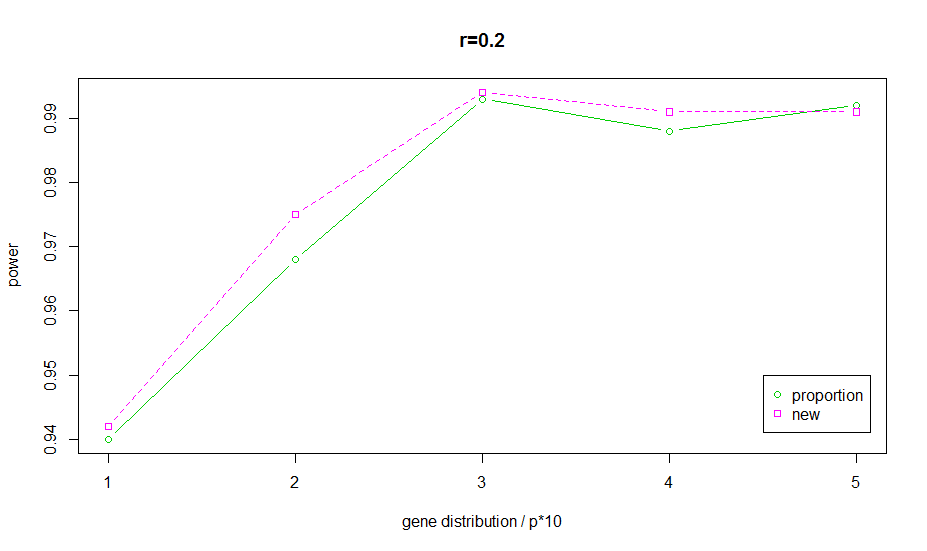
\includegraphics[height = 8cm]{r2.png}
\caption{$r = 0.2$}
\end{figure}

From the results above, we conclude that our new method performs better.

\end{CJK}
\end{document}
